%\documentclass[a4paper,onecolumn,draft]{IEEEtran}
\documentclass[a4paper,onecolumn]{IEEEtran}
\usepackage{amsmath}
\usepackage[english]{babel}
\usepackage{graphicx}
\usepackage{ctable}
\usepackage{url}

\author{A. Bossenbroek}
\title{Lab Report Computational Aspects of Stochastic Differential Equations}

\begin{document}
\maketitle
Assuming the volatility to be constant, as is done in the seminal work by Black
and Scholes, can be too much of a simplification. In this work a stock process
is considered which has a drift term, volatility, modeled as a mean reverting
stochastic process. The stock process is given as:
\newcommand{\indst}{\ensuremath{^{(1)}}}
\newcommand{\indvl}{\ensuremath{^{(2)}}}
\begin{equation}\label{eq:stock}
dS_t = \mu S_t dt + \sigma_t S_t dW_t\indst
\end{equation}
the volatility of the stock is defined to be:
\begin{equation}\label{eq:vol}
d\sigma_t = -(\sigma_t - \xi_t)dt + p\sigma_t dW_t\indvl
\end{equation}
which includes a mean reverting term $\xi_t$ defined as follows:
\begin{equation}\label{eq:mnrvrt}
\xi_t = \frac{1}{\alpha}(\sigma_t - \xi_t)dt
\end{equation}
The Brownian motions $W_t^{\{(1), (2)\}}$ in  equation \eqref{eq:stock} and
\eqref{eq:vol} are two independent identically distributed random variables.
They have the property that $W_0=0$ and $W_t - W_s \sim N(0, t - s)$ for $s <
t$.

\section{Numerical Methods}
\subsection{Stock Process}
To solve the stochastic differential equation (SDE) which models the stock 
process numerically three numerical methods are used. All methods rely on
rewriting the SDE in equation \eqref{eq:stock} to an It\=o process. For this two
auxiliary functions are introduced 
\begin{align}\label{eq:abstck}
a(S_t)&=\mu S_t&b(S_t)&=\sigma_t S_t.
\end{align}
Note that both functions do not include the independent variable $t$.  The
stock process can then be rewritten to:
\newcommand{\inttim}{\ensuremath{\int_{t_0}^{t}}}
\newcommand{\intdel}{\ensuremath{\int_{t}^{t + \Delta t}}}
\begin{equation*}
dS_t = a(S_t)dS_t + b(S_t)dW_t\indst
\end{equation*}
or
\begin{equation*}
S_t = S_0 + \inttim a(S_t)ds + \inttim b(S_t)dW\indst.
\end{equation*}
This value can only be approximated by taking a --infinitesimal-- small step
$\Delta t$ from $t$. The new value $S_{t + \Delta t}$ can be found using
different numerical methods. Three methods are discussed below.

\subsubsection{Euler Method}
The Euler method relies on computing the value of $a$ and $b$ as defined in
equation \eqref{eq:abstck}. For an It\=o process the Euler method is defined as:
\begin{equation}\label{eq:euler}
X_{t + \Delta t} = X_t + a\Delta t + b\Delta W
\end{equation}
where $\Delta t$ is the time step more commonly denoted as $h$ in numerical
mathematics and $\Delta W = \left(W\indst_{t + \Delta t} - W\indst_t\right)$.
Since $\left(W\indst_{t + \Delta t} - W\indst_t\right) =
Z\indst\sqrt{\Delta t}$ where $Z\indst\sim N(0, 1)$ the numerical
approximation can easily be found using the Euler method. Given a step size
$\Delta t$ the new stock value can be computed as:
\begin{align}
S_{t + \Delta t} = S_t + \mu S_t\Delta t + \sigma_t S_t Z\indst\sqrt{\Delta t}
\end{align}
where only $a(S_t)$ and $b(S_t)$ have to be computed, this in contrast to
subsequent methods.


\subsubsection{Milstein Method}
The Milstein method is a second method which can be used to compute the
numerical approximation of a SDE. The functions $a$ and $b$ as defined in
equation \eqref{eq:abstck} are used. In conjunction with these functions, the
Milstein method necessitates also $b'(S_t) = \sigma_t$. For an It\=o process
$X_t$ the Milstein method is defined as:
\begin{equation}\label{eq:mil}
X_{t + \Delta t} = X_t + a\Delta t + b\Delta W +
\frac{1}{2}bb'\left(\left(\Delta W\right)^2 - \Delta t\right)
\end{equation}
with $\Delta t$ and $\Delta W$ as defined before. For the SDE in
equation \eqref{eq:stock} the approximation is:
\begin{equation}
S_{t + \Delta t} = S_t + \mu S_t dt + \sigma_t S_t Z\indst\sqrt{\Delta t} +
	\frac{1}{2} \sigma_t^2 S_t \left(\left(Z\indst\sqrt{\Delta t}\right)^2 -
\Delta t\right)
\end{equation}
In contrast to the Euler method, the Milstein method not only requires to
compute $a(S_t)$ and $b(S_t)$, it also requires $b'(S_t)$.

\subsubsection{Runge-Kutta Method}
For a numerical approximation of a SDE using the Milstein method the
evaluation of $b'$ is necessary. However, in some circumstances $b'$ may be
unavailable or too expensive to compute. Therefore another numerical method
is also used. The Runge-Kutta method only necessitates the evaluation of $a$
and $b$ which similar to the Euler method. For an It\=o process $X_t$ the
Runge-Kutta method is defined as
\begin{equation}\label{eq:rk}
X_{t + \Delta t} = X_t + a\Delta t + b\Delta W + \frac{1}{2\sqrt{\Delta
t}}\left(\left(\Delta W\right)^2 - \Delta
t\right)[b\left(\bar{X_t}\right)-b(X_t)]
\end{equation}
where $\bar{X_t}$ is defined as:
\begin{equation}
\bar{X_t} = X_t + a\Delta t + b \sqrt{\Delta t}
\end{equation}
Applying this method to the stock process defined in equation \eqref{eq:stock}
the Runge-Kutta approximation can be computed as:
\begin{equation}
\begin{split}
\bar{S_t} &= S_t + \mu S_t\Delta t + \sigma_t S_t \sqrt{\Delta t}\\
S_{t + \Delta t} &= S_t + \mu S_t \Delta t + \sigma_t S_t Z\indst\sqrt{\Delta
t} + \frac{1}{2\sqrt{\Delta t}}\left(\left(Z\indst\sqrt{\Delta t}\right)^2 -
\Delta t\right)[\sigma_t\bar{S_t} - \sigma_t S_t]
\end{split}
\end{equation}
using this method the computational times can be decreased.

\subsection{Volatility Process}
In the previous section the numerical approximation of the stock process as
defined in equation \eqref{eq:stock} was discussed. In this section we will
discuss how the numerical approximation of the volatility process as defined
in equation \eqref{eq:vol} can be approximated. As with the stock process three
different numerical methods will be used. Since we already defined the Euler
method (see equation \eqref{eq:euler}), Milstein method (see equation
\eqref{eq:mil}) and Runge-Kutta method (see equation \eqref{eq:rk}) for an
It\=o process, this section will only discuss the applications of these
methods on the volatility process. For each approximation method we define $a$
and $b$ as follows:
\begin{align}
a(\sigma_t)&= -(\sigma_t - \xi_t) & b(\sigma_t) = p\sigma_t
\end{align}
The approximation of the volatility process using the Euler method can be
found with:
\begin{equation}
\sigma_{t + \Delta t} = \sigma_t - (\sigma_t - \xi_t)\Delta t +
	p\sigma_tZ\indvl\sqrt{\Delta t}
\end{equation}
where $Z\indvl\sim N(0, 1)$ is independent from $Z\indst$.

The approximation of the volatility process using the Milstein method can be
found with:
\begin{equation}
\sigma_{t + \Delta t} = \sigma_t - (\sigma_t - \xi_t)\Delta t +
	p\sigma_t Z\indvl \sqrt{\Delta t} + \frac{1}{2}p^2\sigma_t 
	\left(\left(Z\indvl\sqrt{\Delta t}\right)^2 - \Delta t\right)
\end{equation}

The Runge-Kutta method for the approximation of the volatility process is:
\begin{equation}
\begin{split}
\bar{\sigma_t} &= \sigma_t  -(\sigma_t - \xi_t)\Delta t + p\sigma_t 
	\sqrt{\Delta t}\\
\sigma_{t + \Delta t} &= \sigma_t - (\sigma_t - \xi_t)\Delta t 
	+ p\sigma_t Z\indvl\sqrt{\Delta t}
	+ \frac{1}{2\sqrt{\Delta t}}\left(\left(Z\indvl\sqrt{\Delta t}\right)^2 -
\Delta t\right)[p\bar{\sigma_t} - p\sigma_t]
\end{split}
\end{equation}

\subsection{Mean-Reverting Term}
A feature of the volatility process defined in equation \eqref{eq:vol} is that
it is mean reverting. The definition of the mean reverting term is given in
\eqref{eq:mnrvrt}. Since this function is deterministic the previous
stochastic approximation methods cannot be used. However, the numerical
approximation is essential. In subsequent sections the approximation error of
each individual stochastic numerical approximation will be the center of our
investigation. To reduce the approximation error originating from the
numerical integration of the mean reverting process a fourth-order
approximation method is used.  The Runge-Kutta numerical approximation method
(from this point forward revert to as the RK4) for the ordinary differential
equation defined in equation \eqref{eq:mnrvrt} is:
\begin{equation}
\xi_{t + \Delta t} = \xi_t + \frac{\Delta t}{6}(k_1 + 2k_2 + 2k_3 + k_4)
\end{equation}
where $k_{\{1, 2, 3, 4\}}$ are defined as:
\begin{align*}
k_1 &= \frac{1}{\alpha}(\sigma_t - \xi_t)\\
k_2 &= \frac{1}{\alpha}\left(\left(\sigma_t + \frac{\Delta t}{2}k_1\right) -
	\xi_t\right)\\
k_3 &= \frac{1}{\alpha}\left(\left(\sigma_t + \frac{\Delta t}{2}k_2\right) -
	\xi_t\right)\\
k_4 &= \frac{1}{\alpha}\left(\left(\sigma_t + \Delta t k_3\right) -
	\xi_t\right)
\end{align*}
With this last numerical approximation it is possible to implement the methods
in an algorithm and find solutions.

\section{Experiments}
Various experiments were conducted by means of computer programs which
implement the numerical approximations methods discussed in the previous
section. The first experiments investigate the impact of $p$ and $\alpha$ on
the behaviour of $S_{0 \leq t \leq T}$, $\sigma_{0 \leq t \leq T}$ and
$\xi_{0 \leq t \leq T}$. The second investigates the order of strong order of
convergence of each method. The last experiments are conducted to observe the
weak order of convergence.

\newcommand{\stockplotsize}{9cm}
\ctable[caption={The path of a stock given different $p$ for $\alpha = \{0.1,
				1, 2\}$},
		 label={fig:stockpath},
		 figure]{cc}{\tnote[]{$\quad$In each figure shows six realizations of a stock
		 path. The path is modeled with the model in equation \eqref{eq:stock}.
		 The parameters which are equal in each figure are $S_0 = 50$, $\mu =
		 0.2$, $\xi_0 = 0.2$, $\sigma_0=0.2$, $T=1$ and $\Delta t = 0.0001$. The left
		 column shows realizations of the path which a different state of the
		 Mersenne Twister random number generator \cite{matsumoto1998mtd}. The
		 left column uses state 12 to generate $Z^{(1)}$ and 13 to generate
		 $Z^{(2)}$. The right column uses state 2 and 3 for both random number
		 sequences. Each row uses a different $\alpha$ in the mean reverting
		 term $\xi_t$ as defined in equation \eqref{eq:mnrvrt}.\\
		 $\quad$In the left column the results show that increasing the
		 diffusion term of the volatility ($p$) leads for all $\alpha$ to a
		 reduction of the drift of the process. This also holds for the results
		 in the right column for $p=4$. However only for small time periods ($0.4<t<0.5$
		 and $(0.75<t<1)$). Furthermore, the right column shows that when $p=2$
		 the stock has a higher volatility than when $p=0.01$. This in contrast
		 to the left column. There $p=0.01$ has the highest volatility.
		 $\quad$The impact of $\alpha$ on the stock process is best seen in the
		 left column. Increasing $\alpha$ causes the volatility of the stock for
		 $p= 2, 4$ to augment. However, only marginally in the left column. In
		 the right column the volatility of the stock process when $p=4$ is
		 considerable larger at a higher $\alpha$ (compare the three rows at
		 $0.55<t<0.7$)
		 }}{\FL
		 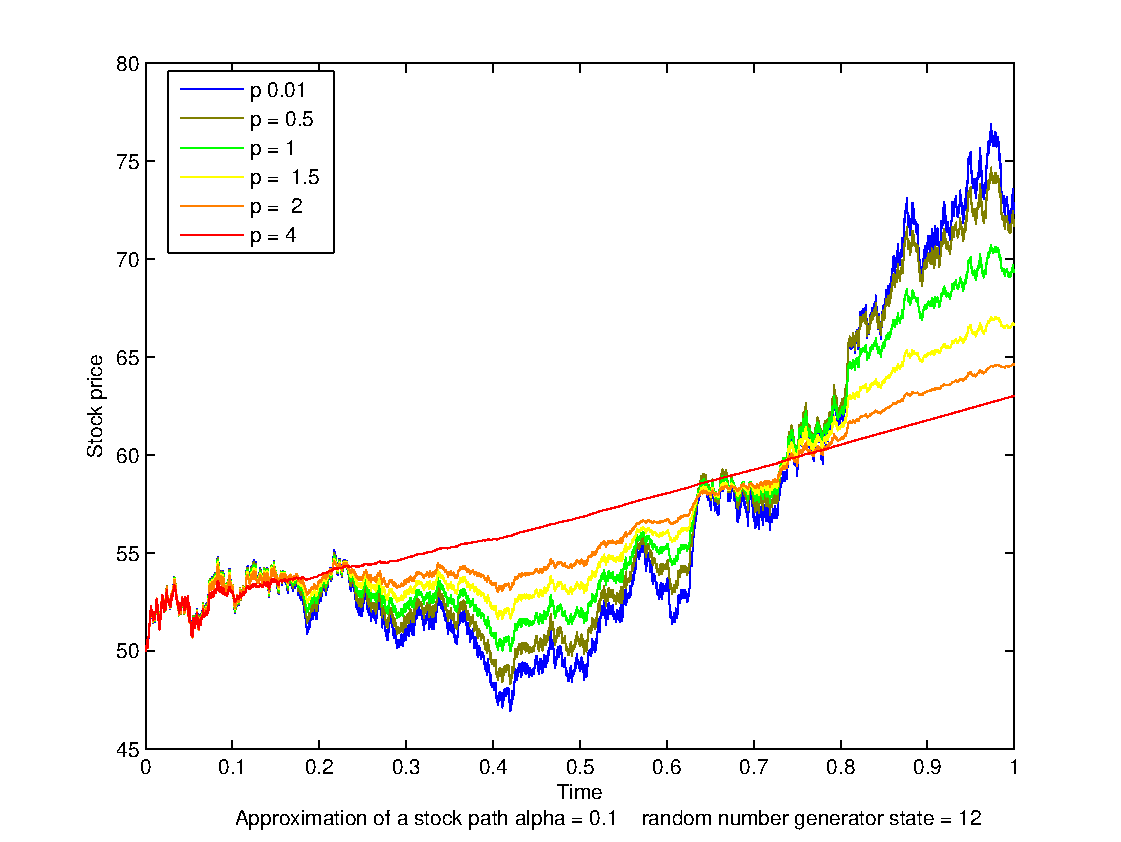
\includegraphics[width=\stockplotsize]{stock_alpha0-1}&
			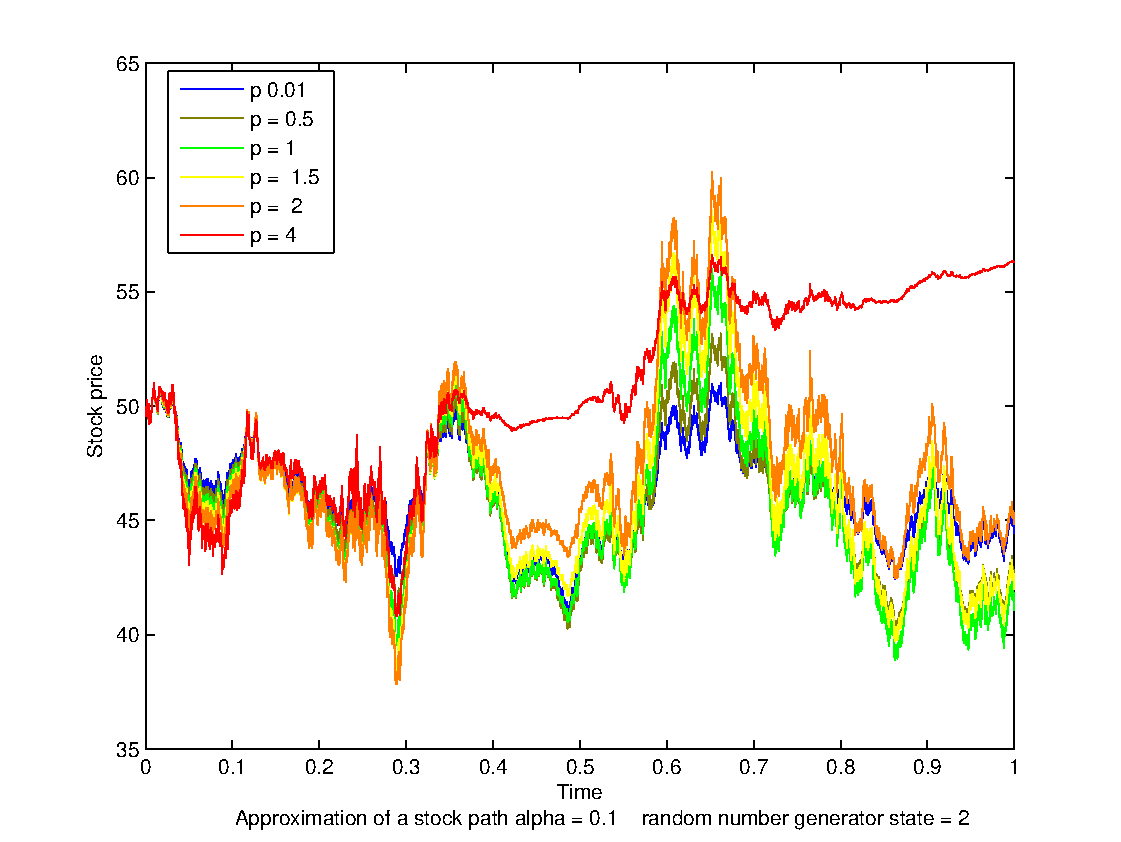
\includegraphics[width=\stockplotsize]{stock_s2_alpha0-1}\NN\cmidrule(lr){1-2}
		 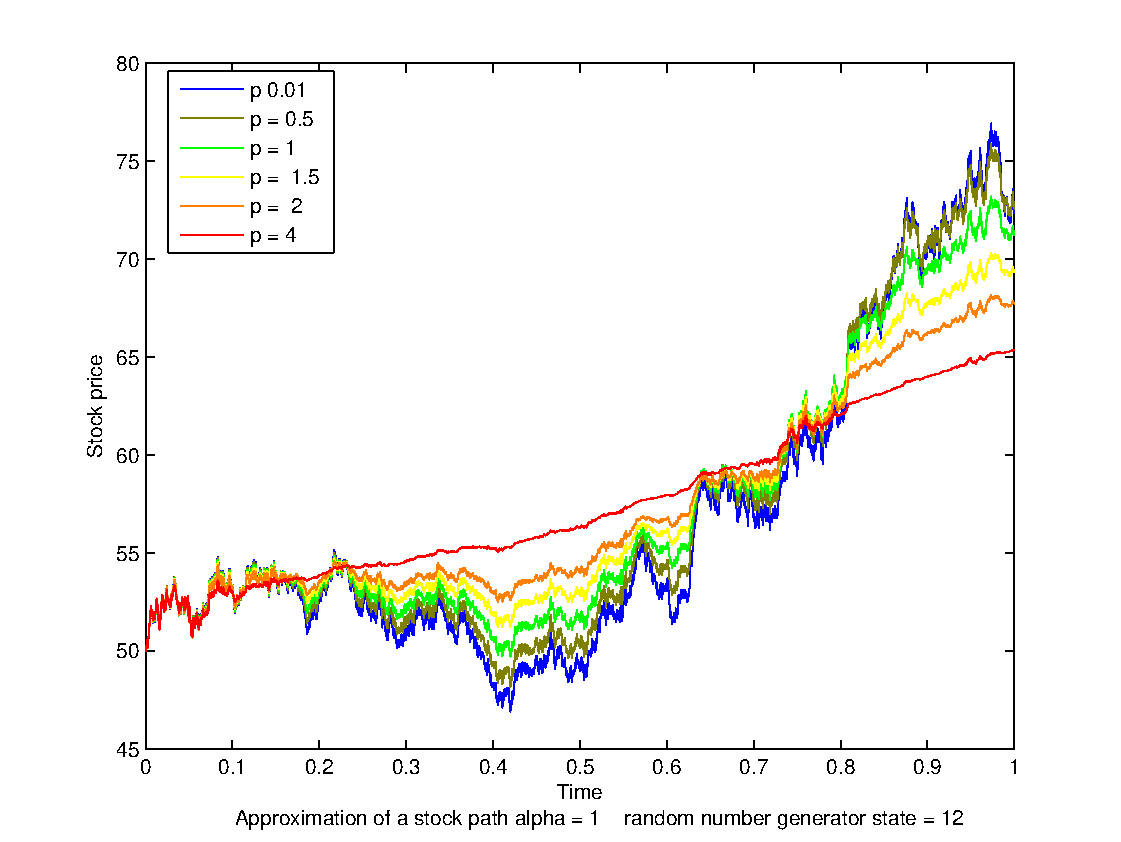
\includegraphics[width=\stockplotsize]{stock_alpha1}&
			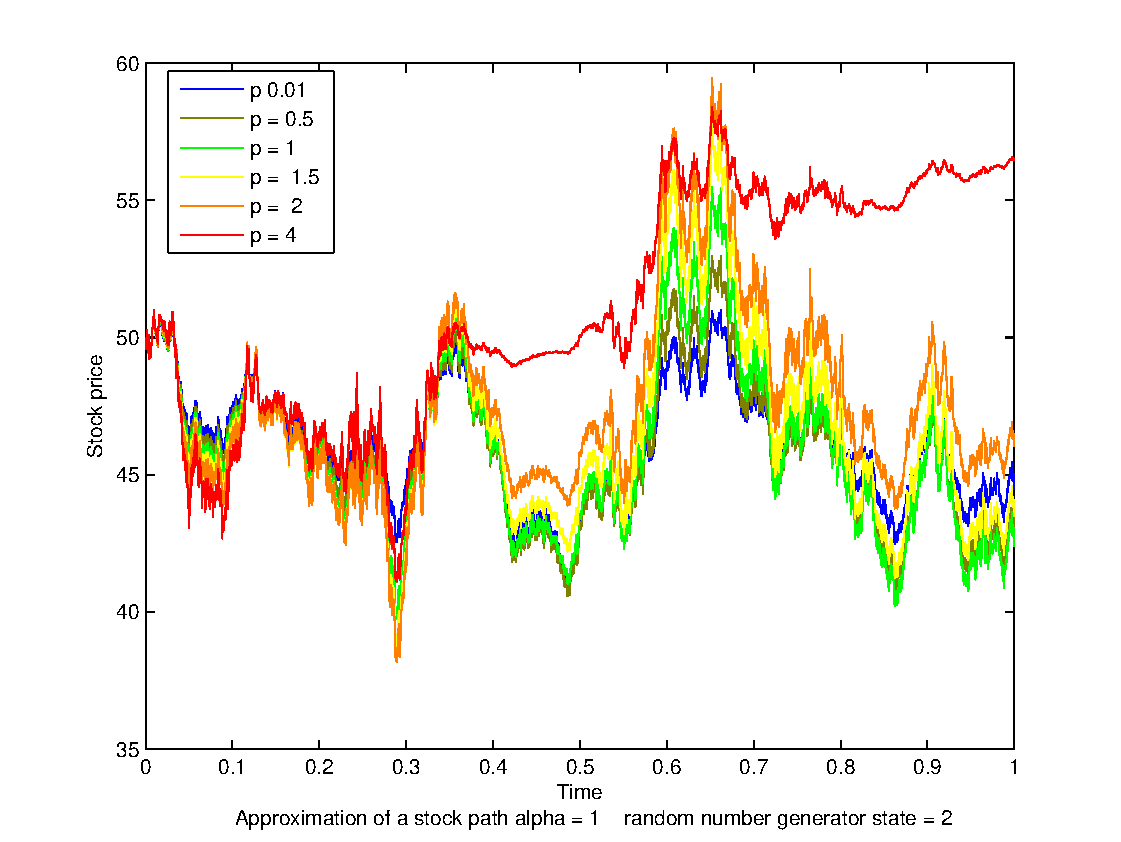
\includegraphics[width=\stockplotsize]{stock_s2_alpha1}\NN\cmidrule(lr){1-2}
		 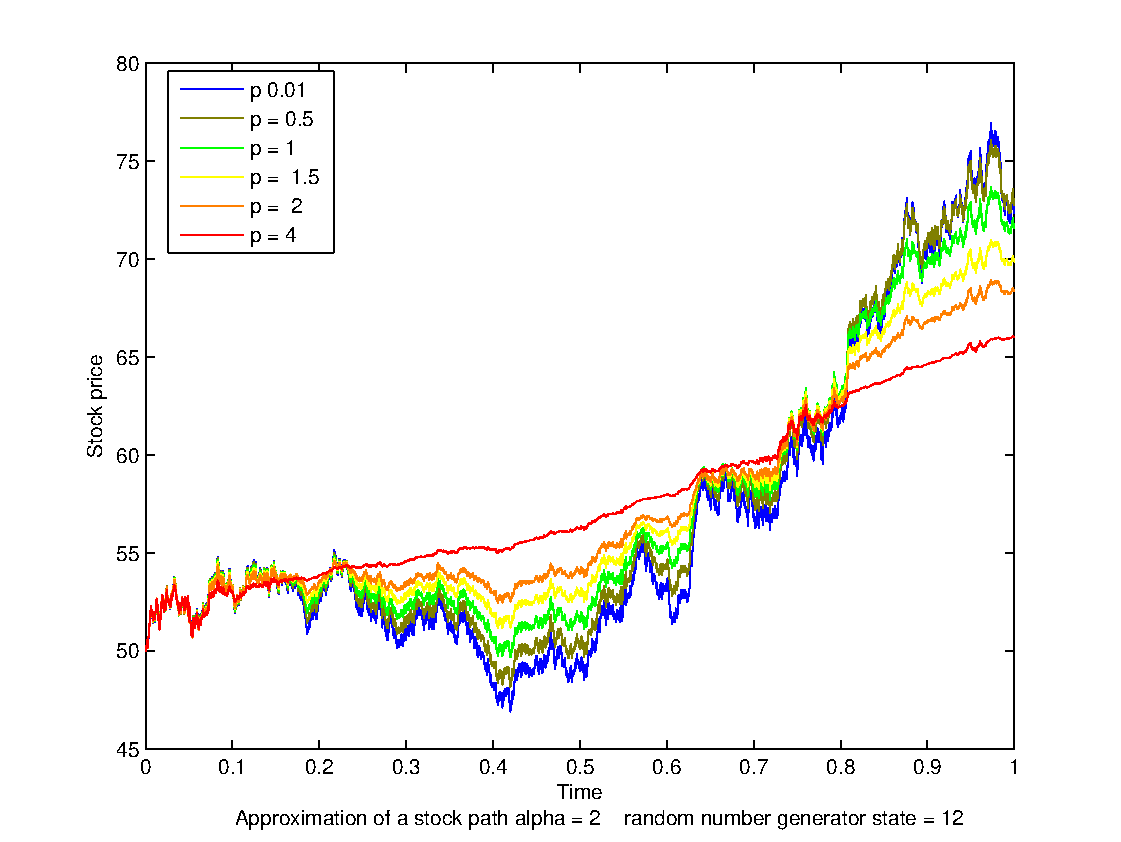
\includegraphics[width=\stockplotsize]{stock_alpha2}&
			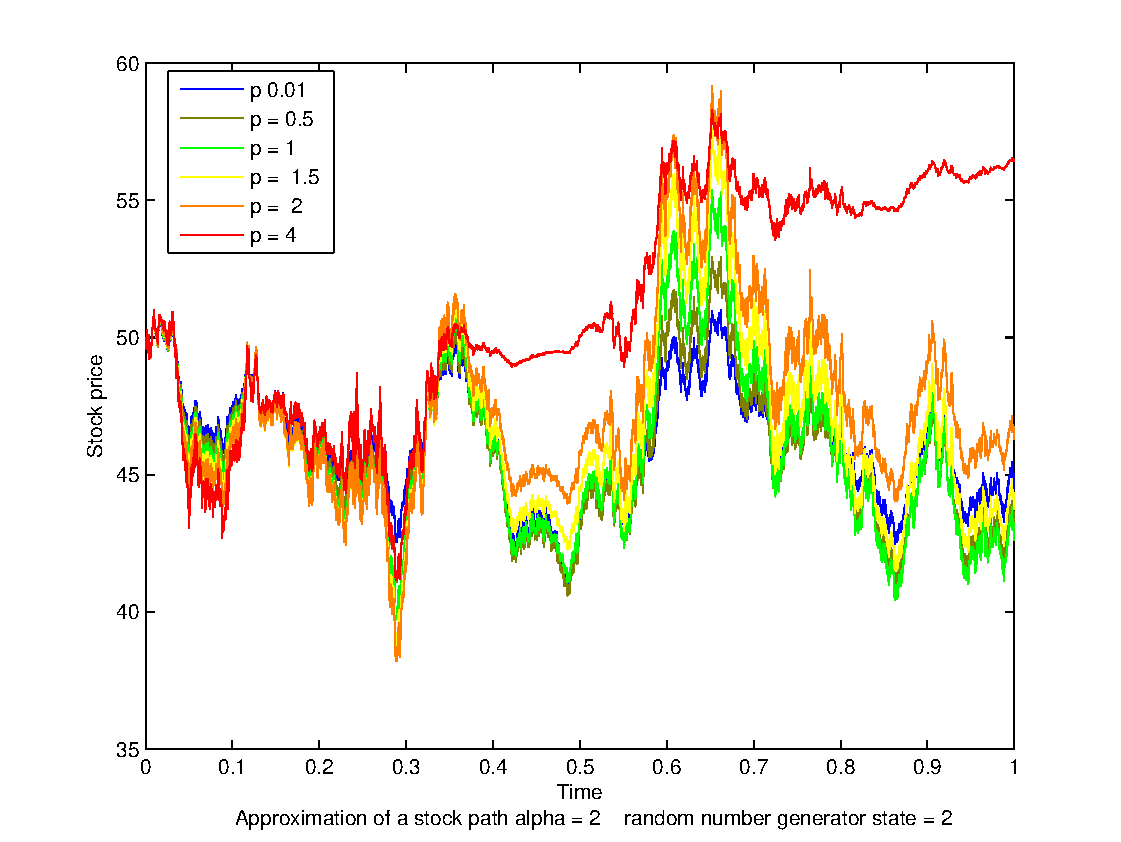
\includegraphics[width=\stockplotsize]{stock_s2_a2}\LL
			}
		
\ctable[caption={Several realizations of the stock - and volatility process
				and $\xi_t$ for different combinations of $p$ and $\alpha$.},
		 label={fig:svxpaths},
		 figure]{cc}{\tnote[]{This figure displays six triples figures showing
		 30 realizations of the stock path, volatility path and $\xi_t$ path. The
		 constant parameters of the model are the same as in figure
		 \ref{fig:stockpath}. The initial state of the Mersenne Twister random
		 number generator for $Z^{(1)}$ 1 and 2 for $Z^{(2)}$. From top to bottom the rows have
		 $p = 0.5, 1$ and $2$. The left and right column have respectively
		 $\alpha = 0.1$ and $\alpha = 2$.\\
		 $\quad$Increasing $\alpha$ in the mean reverting term damps
		 down $\xi_t$. The impact of $\alpha$ on the volatility is less obvious.
		 The gray line which represents one of the volatility paths in the top
		 row shows that an increase of $\alpha$ leads to a lower maximum. The
		 same conclusion can be drawn when looking at the red line which
		 represents a realization of the volatility in the middle row. Since the
		 effect on the volatility is marginal, the effect will be even smaller
		 on the stock price process.\\
		 $\quad$An increase of $p$ shows that the diffusion of the
		 volatility and thereby also the stock price. In the bottom row the
		 volatility process shows very volatile behaviour which is also 
		 recognizable in the stock process. However the impact is not as
		 significant on each process. The brown stock price realization
		 oscillates considerably more at a higher $p$, the purple process
		 however displays behaviour identical to the process in figure
		 \ref{fig:stockpath}.
		 }}{\FL
		 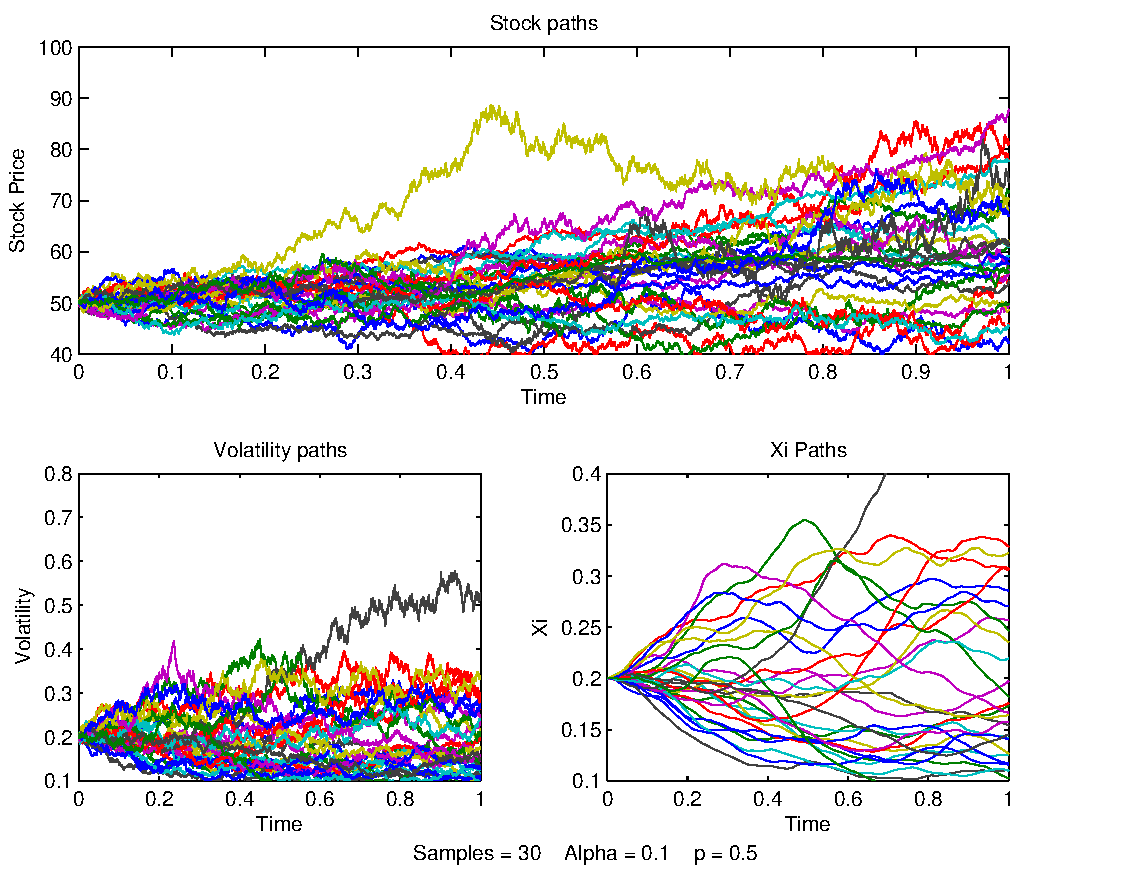
\includegraphics[width=\stockplotsize]{path_s30_a0-1_p0-5}&
			 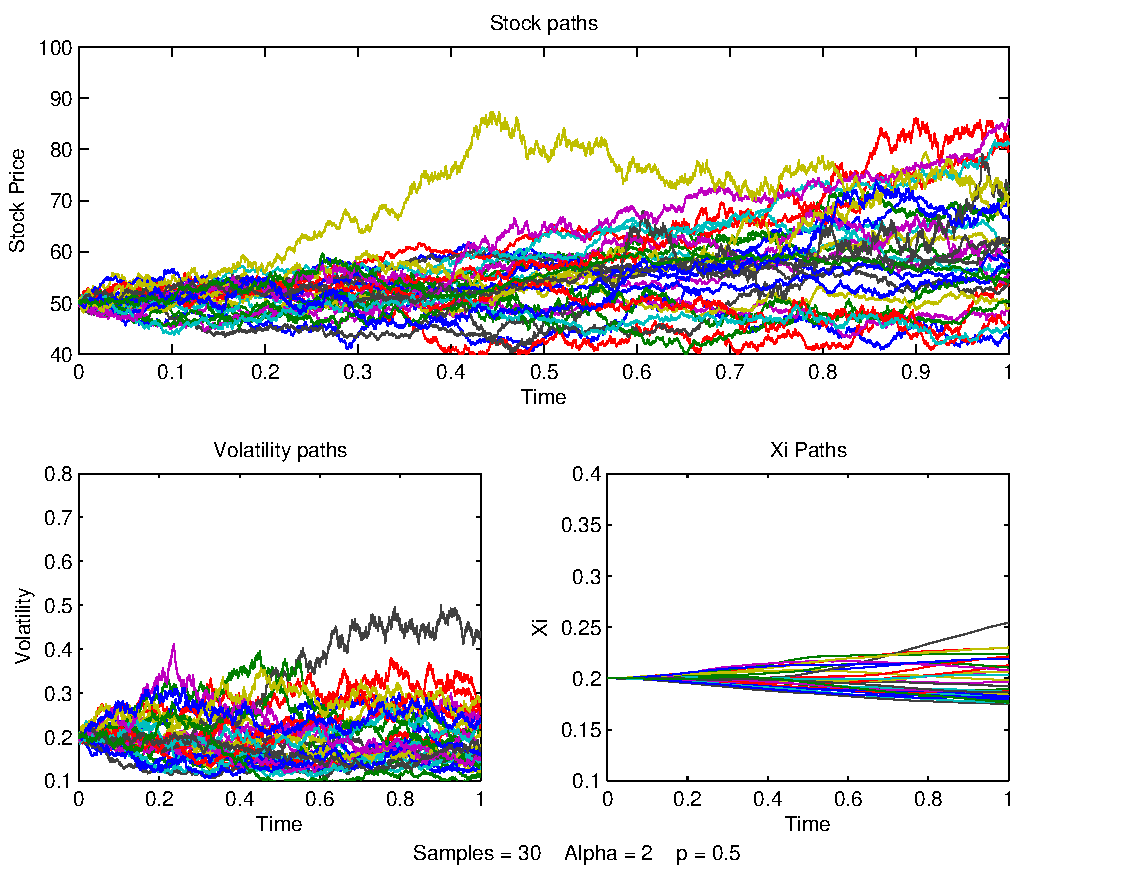
\includegraphics[width=\stockplotsize]{path_s30_a2_p0-5}\NN\cmidrule(lr){1-2}
		 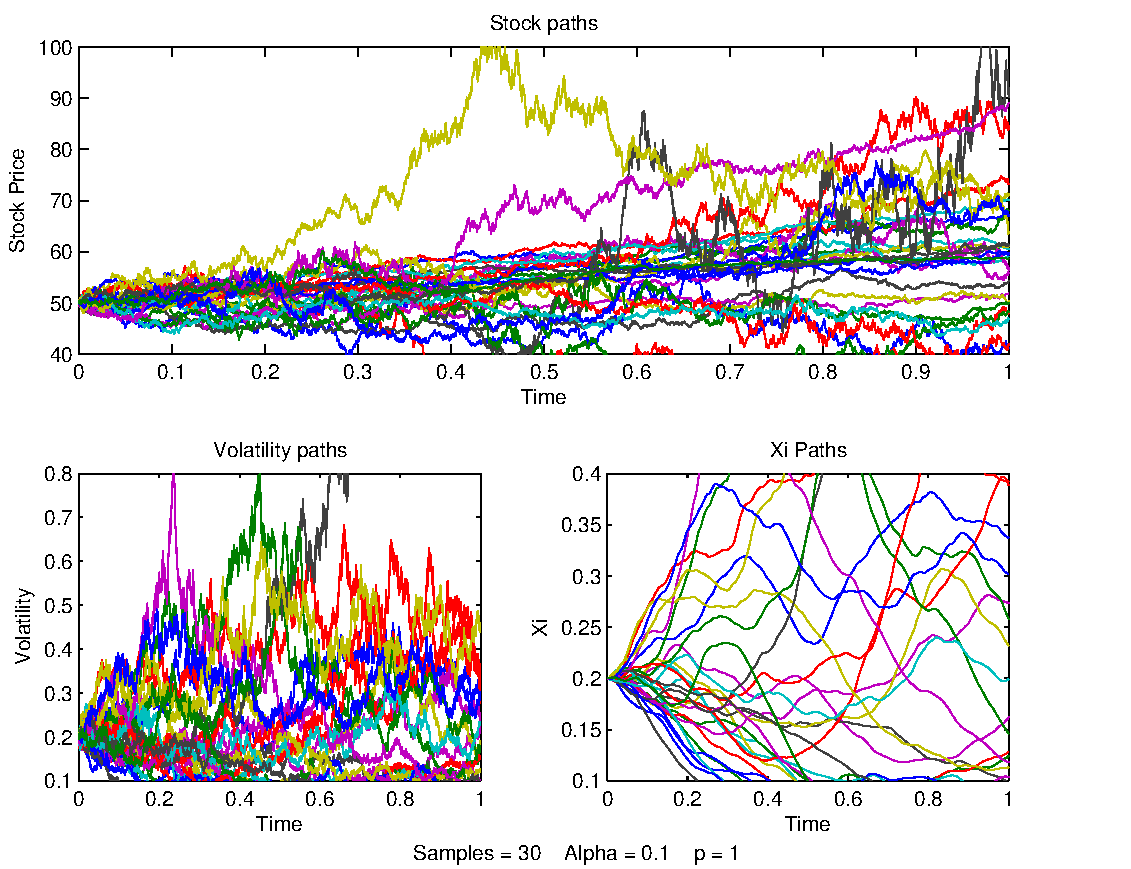
\includegraphics[width=\stockplotsize]{path_s30_a0-1_p1}&
			 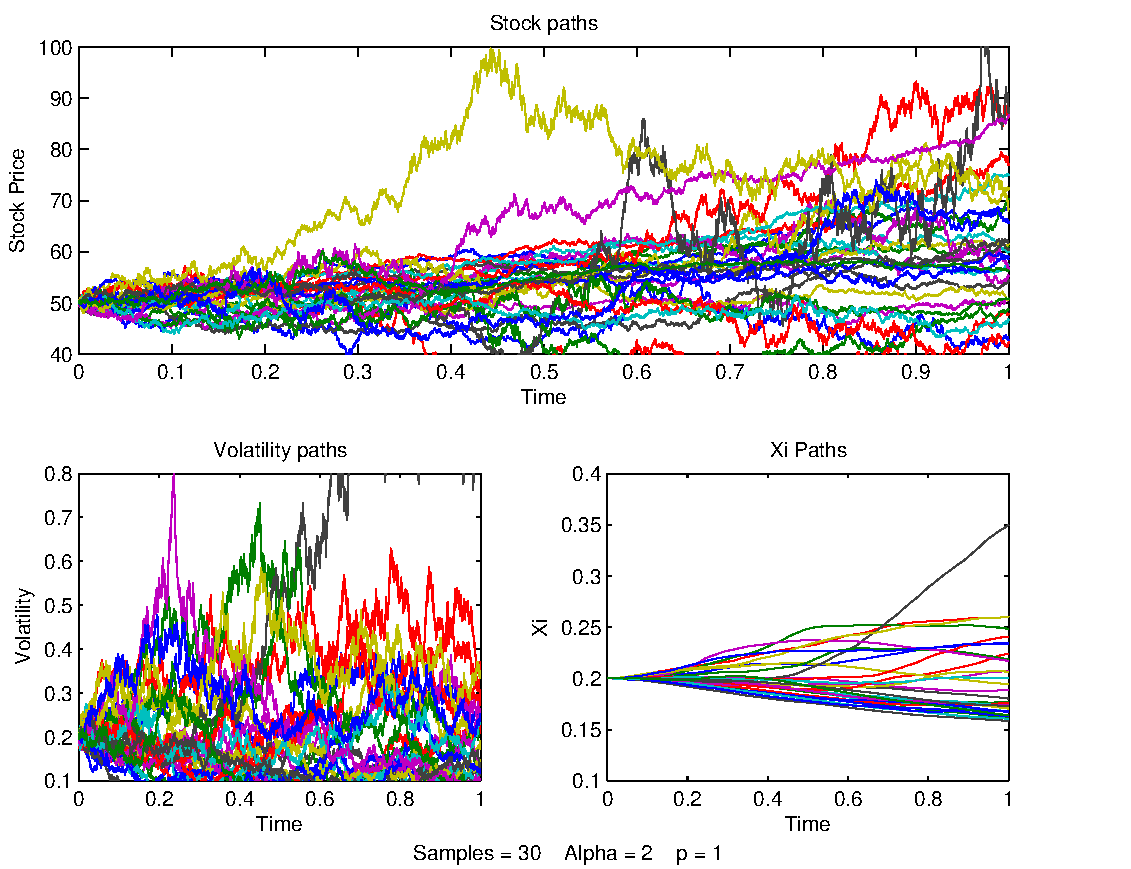
\includegraphics[width=\stockplotsize]{path_s30_a2_p1}\NN\cmidrule(lr){1-2}
		 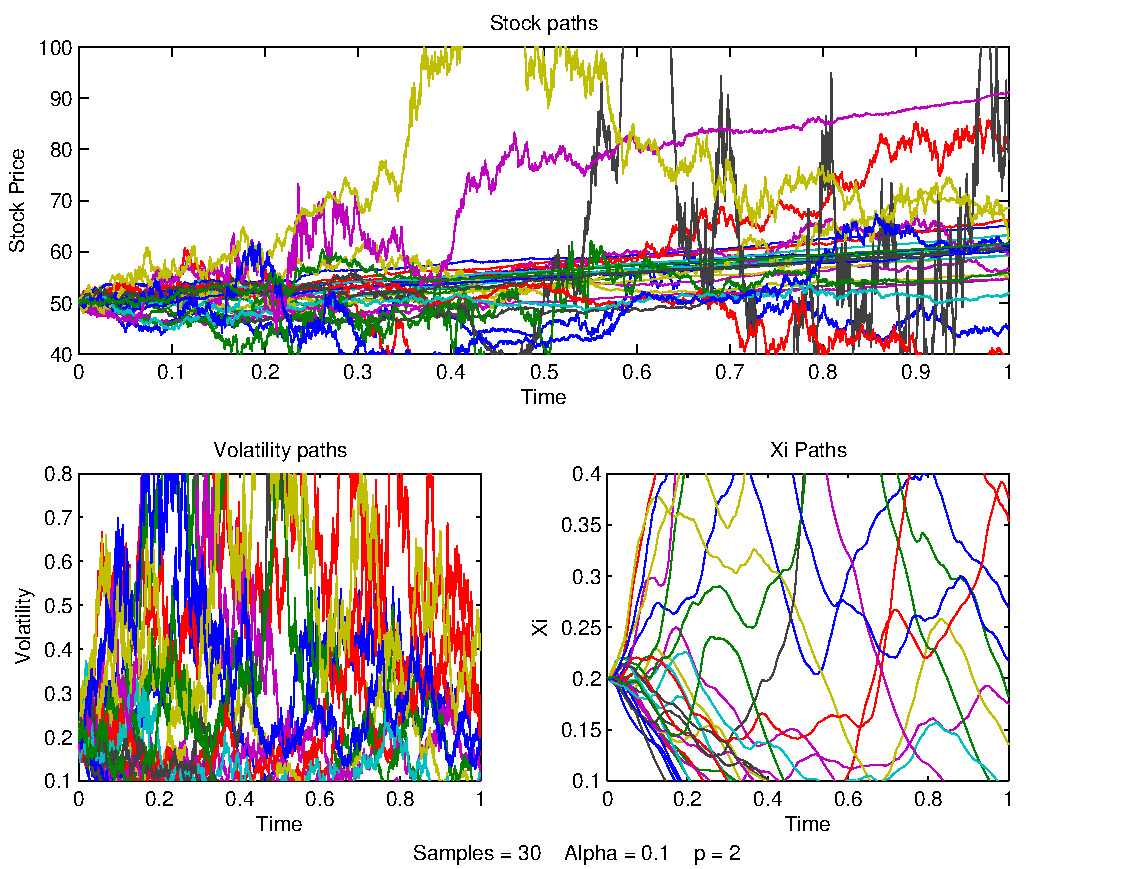
\includegraphics[width=\stockplotsize]{path_s30_a0-1_p2}&
			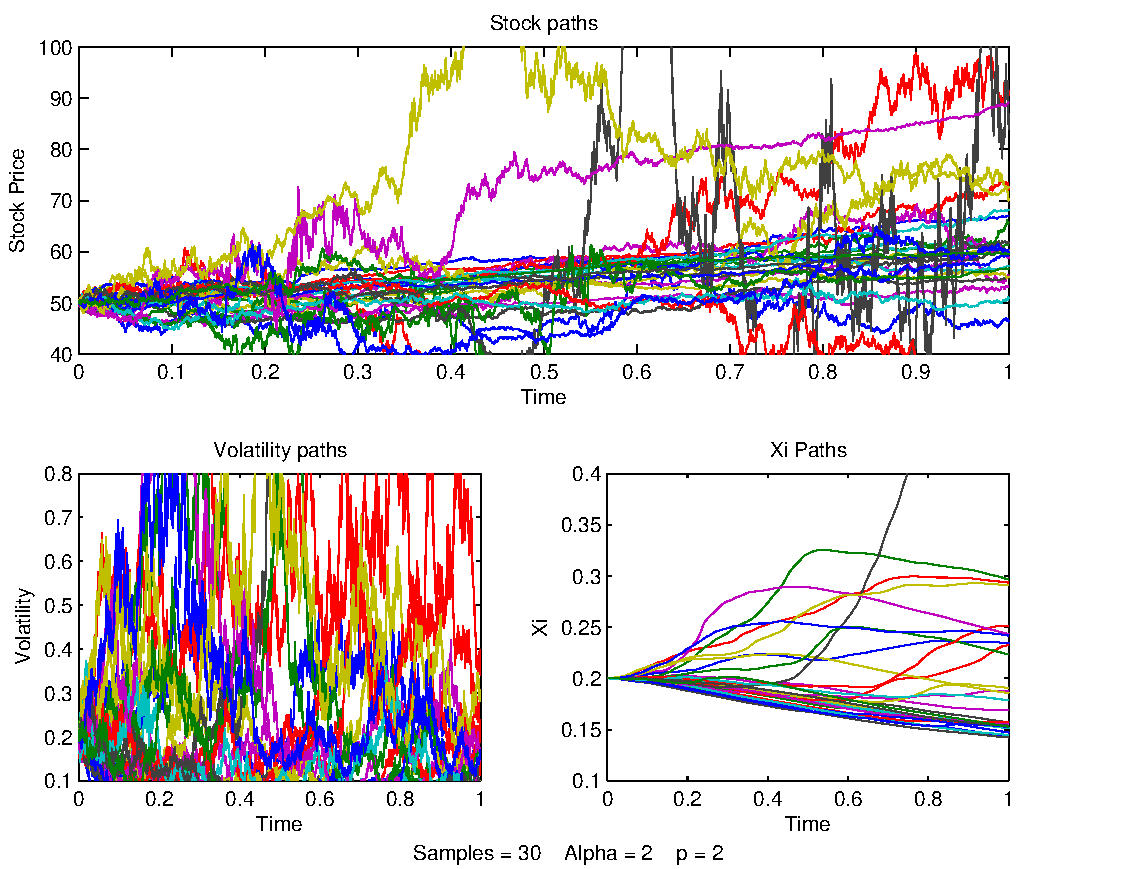
\includegraphics[width=\stockplotsize]{path_s30_a2_p2}\LL
			}

\ctable[caption={Box plot of the volatility and stock price at five points in
				time for various $\alpha$ and $p$.},
		 label={fig:box},
		 figure]{cc}{\tnote[]{$\quad$This figure displays six pairs of box
		 plots. Each pair consists of a box plot of the stock price at five
		 points in time and a box plot of the volatility at five points in time.
		 The constant parameters of the model are the same as in figure
		 \ref{fig:stockpath}. The initial state of the Mersenne Twister random
		 number generator for $Z^{(1)}$ 1 and 2 for $Z^{(2)}$. The data is the
		 same as in figure \ref{fig:svxpaths}. From top to bottom the rows have
		 $p = 0.5, 1$ and $2$. The left and right column have respectively
		 $\alpha = 0.1$ and $\alpha = 2$.\\
		 $\quad$ The red line in each box shows the mean of the data. The bottom
		 of the box shows the value of the first quartile. The top of the box
		 shows value of the third quartile. The whiskers display the upper and
		 lower bound using the interquartile range. The red crosses are
		 outliers.\\
		 $\quad$Considering the size of the boxes and the whiskers in the top
		 row shows that a low diffusion term leads to very few outliers.
		 Moreover, an increase of $\alpha$ at a $p=0.5$ leads the data to be
		 less spread (the whiskers are shorter in the right column than in the
		 left column). Increasing the diffusion term of the volatility leads the
		 data to be more spread out for both, the stock price and the
		 volatility. This is best seen in the bottom row where the boxes are
		 very small and many outliers exist. Lastly, in each volatility plot it
		 is clear that the mean that most the points are above the mean. This
		 spread is consistent with a log-normal distribution.}}{\FL
		 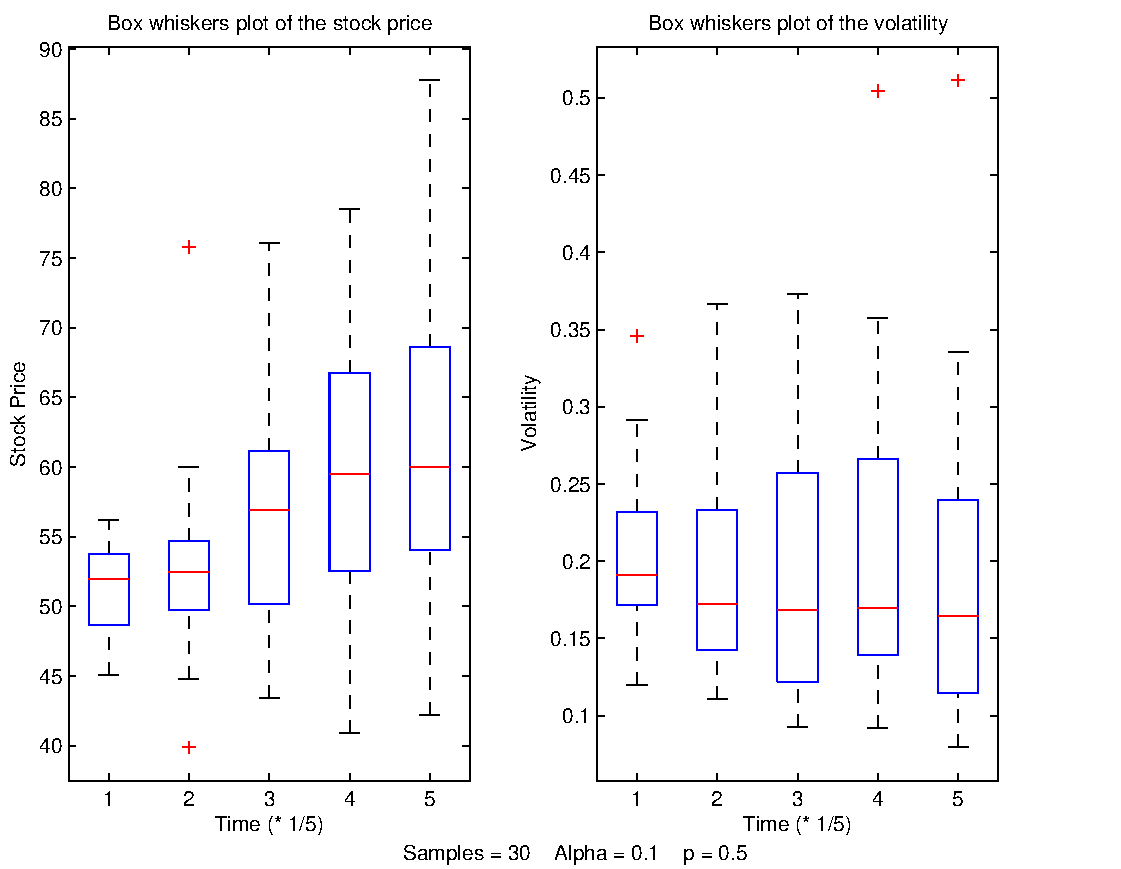
\includegraphics[width=\stockplotsize]{box_s30_a0-1_p0-5}&
			 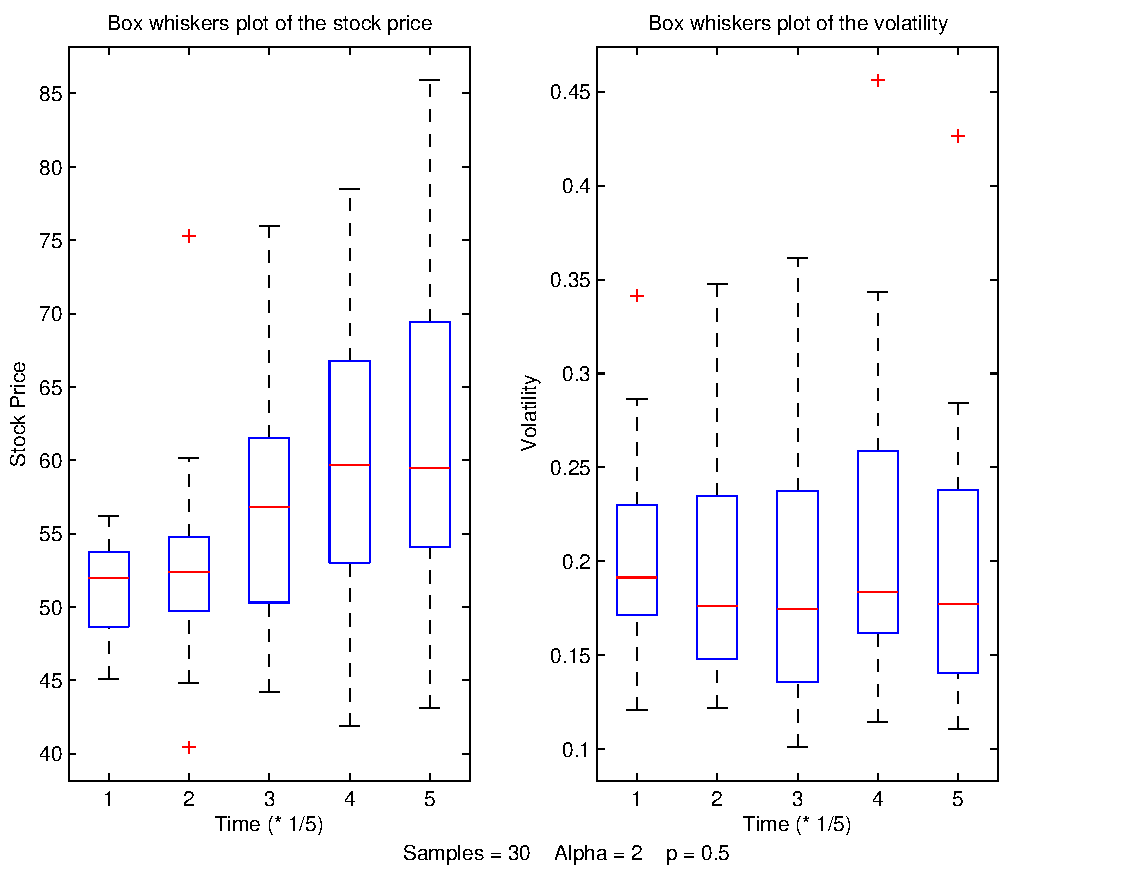
\includegraphics[width=\stockplotsize]{box_s30_a2_p0-5}\NN\cmidrule(lr){1-2}
		 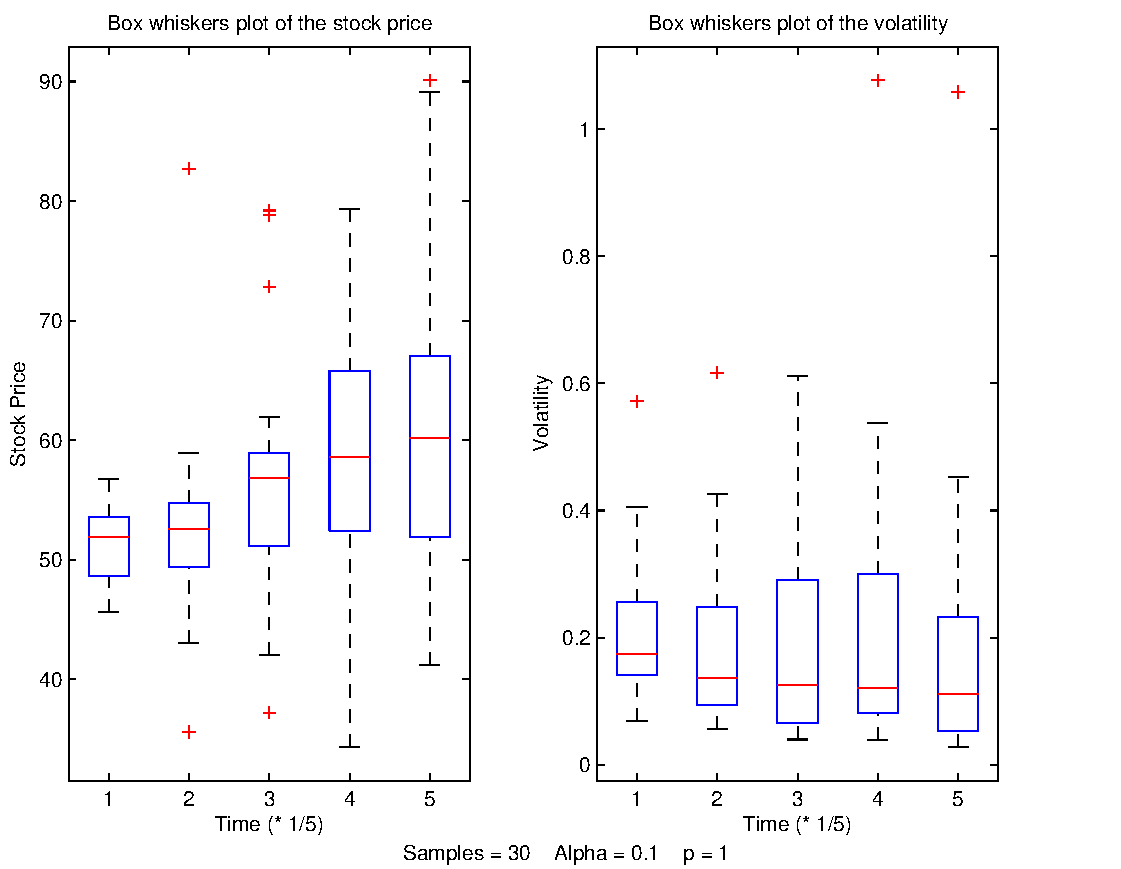
\includegraphics[width=\stockplotsize]{box_s30_a0-1_p1}&
			 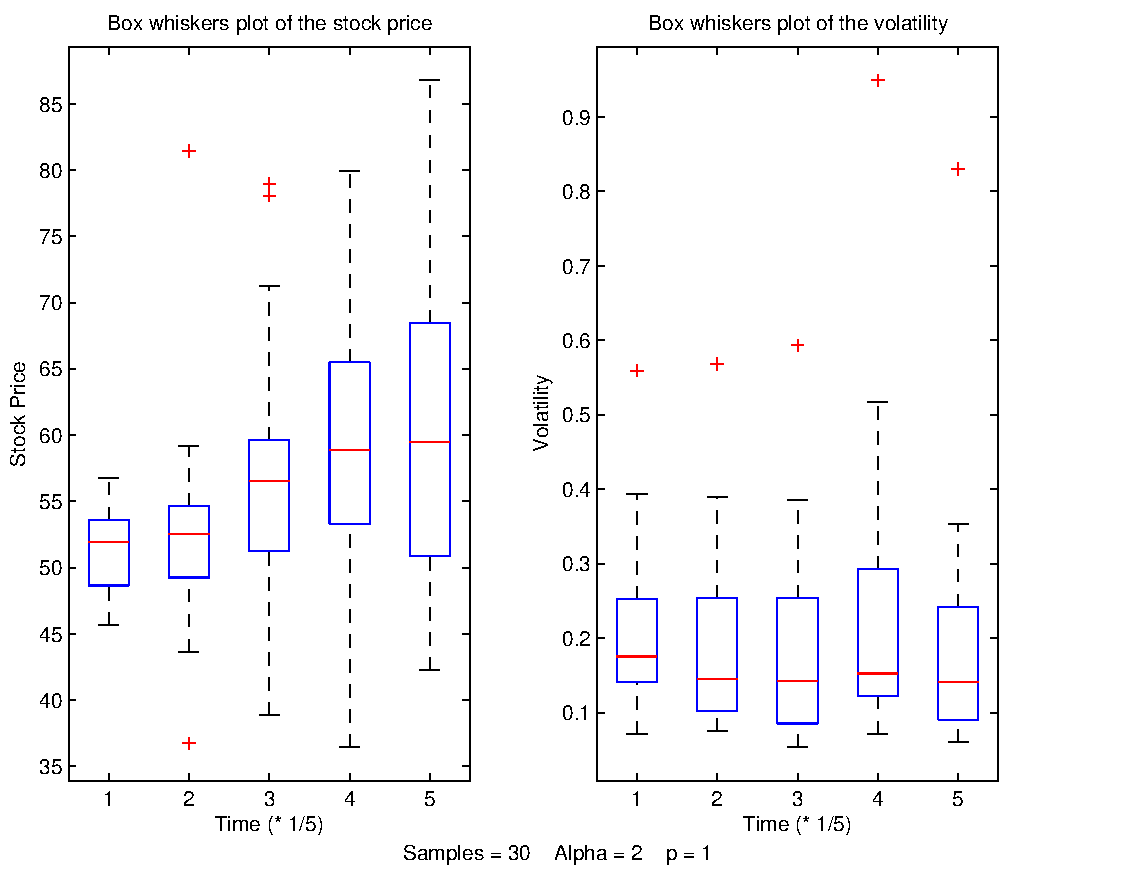
\includegraphics[width=\stockplotsize]{box_s30_a2_p1}\NN\cmidrule(lr){1-2}
		 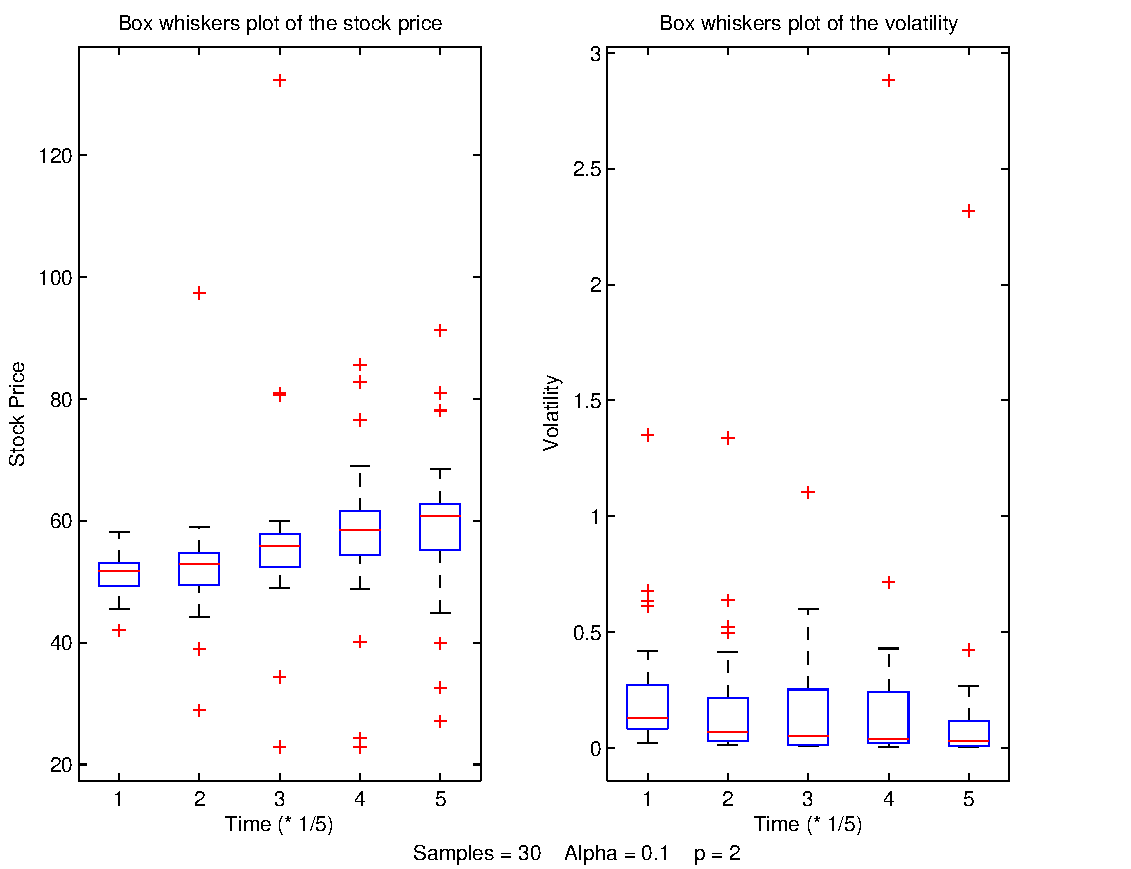
\includegraphics[width=\stockplotsize]{box_s30_a0-1_p2}&
			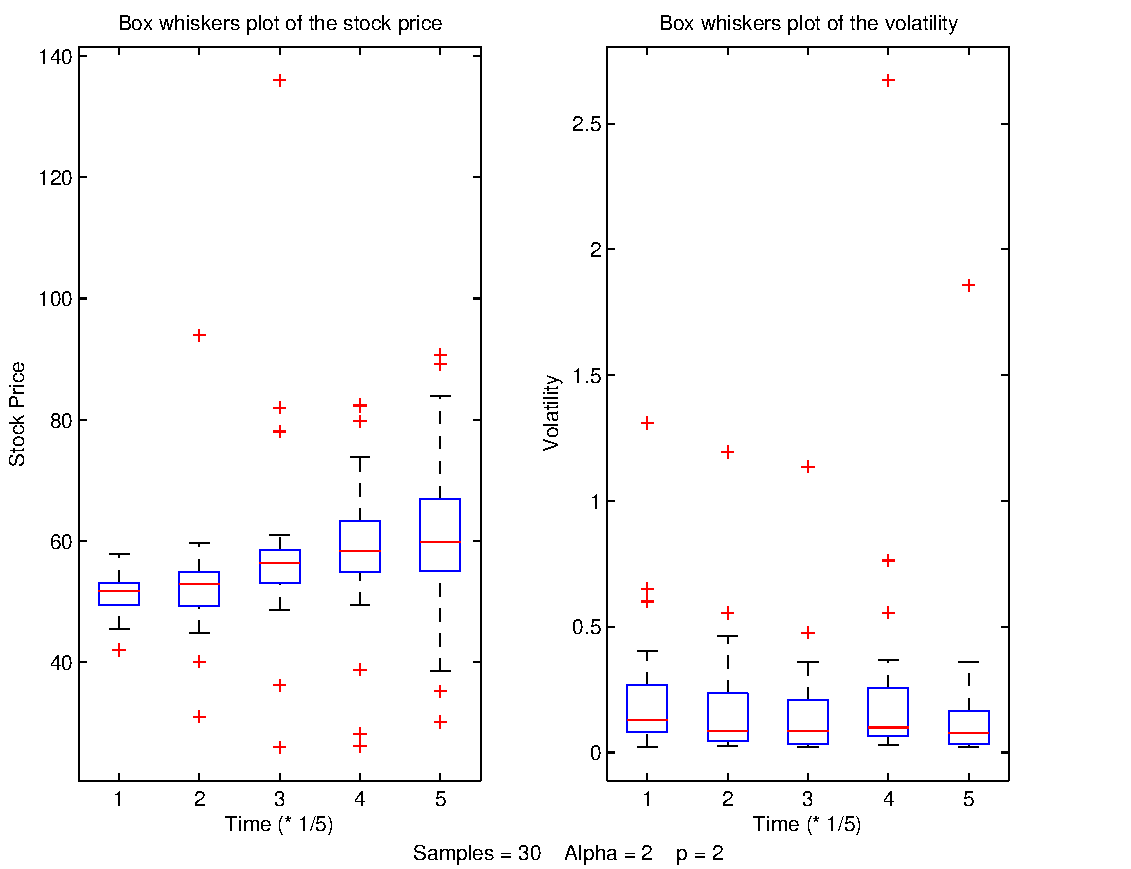
\includegraphics[width=\stockplotsize]{box_s30_a2_p2}\LL
			}


\subsection{Process Behaviour}
In the stock price model which is central to this work the drift term of the
stock is $\mu$ and the diffusion term $\sigma_t$ is modeled as a stochastic
process. The diffusion term consists of a diffusion term which is dependent on
the mean of the process, $\xi_t$, and the diffusion $p$. The mean reverting
term $\xi_t$ includes a `smoothing' term $\alpha$. Two separate experiments
are run to study how the stock, volatility and mean reverting processes are
influenced by $\alpha$ and $p$. The first experiment is conducted to show the
impact of both parameters on a single stock process. The second demonstrates
how not only the stock process is influenced but also the two other processes.
Furthermore, the second study investigates several processes which permits to
draw more general conclusions.

The impact of $\alpha$ and $p$ on one realization of stock path is displayed
in figure \ref{fig:stockpath}. In each column a stock process is shown which has
the same sequence of normally distributed random number $Z^{(1)}_{1\leq t\leq
N}$ and $Z^{(2)}_{1\leq t\leq N}$. The difference is that each process has
different values for the two parameters which effect are being investigated.
From the figure can be concluded that an increase of the diffusion of the
volatility does not lead to an increase of the volatility of the stock
(volatility in the statistical sense and not in the sense of the model).
Comparing the movement of the stock process at a small $\alpha$ leads clearly
to less `spiky' paths. Especially the paths with a high diffusion term in the
volatility are more likely to smoothen when $\alpha$ decreases. We argue that
this is due to the fact that whenever $p$ is low the mean reverting term
$\xi_t$ remains constant and therefore the volatility remains also more
constant (note, $p$ is low). This leads the stock process to change only
marginally when $\alpha$ changes.

The figure also shows that the influence of the parameters is not the same for
all stock processes; the left process appears to converge to a process which
is mainly driven by drift whereas the right process looses its volatility only
locally.  However, also in the right figure increasing $p$ leads the process
to follow the drift more (compare with the processes with a low $p$ which
decrease over time instead of drifting upwards).

As discussed the impact of $\alpha$ and $p$ on the path of process is very
dependent on the sequence of random numbers with which the stock - and the
volatility path are generated. We argue that to be able to reason more in
general more realizations are needed. In figure \ref{fig:svxpaths} six triples
of a stock -, volatility and $\xi_t$ path are displayed for 30 processes. From
the figures which display the path of $\xi_t$ it becomes evident that always
reduces the diffusion of the mean reverting term. There is however no
considerable impact on the stock price. The behaviour of the stock price
changes considerably when $p$ is increased. An increase of this diffusion term
can lead to erratic movement of the volatility and thereby provoke stock
prices to be very volatile.

The values of the volatility - and the stock process are indexed at five
points in time. These values are grouped to construct box plots as shown in
figure \ref{fig:box}. These figures show that at a low $p$ most values can be
grouped in the second and third quartile and that few outliers exist. This is
in stark contrast to the case where $p$ is relatively high. Here the
difference between the second and third quartile is much smaller (the box is
smaller) and the many outliers exist (red crosses). This confirms the
statement we made in the previous paragraph. Furthermore, the plots of the
stock price show that the spread increases over time. This in contrast to the
volatility which remains more less constant. We argue that this is caused by
the mean reverting term. Although it was not obvious in figure
\ref{fig:stockpath} or \ref{fig:svxpaths} the average stock price follows the
drift term $\mu$ (see the red lines in the boxes).


\subsection{Strong Convergence}
Through experiments the order of strong convergence is sought. The three
numerical methods are implemented and tested with several step sizes. The
strong order order of convergence is defined as:
\begin{equation}\label{eq:strng}
\lim_{h\rightarrow 0}(S_T - y_T^h) = O(h^\gamma)
\end{equation}
where $S_T$ is the analytic solution and $y_T^h$ is the approximation using
step size $h$. Since no analytical solution is at hand the value for $S_T$ is
approximated by using the numerical method with an infinitesimal step size of
$h = 0.0001$. To test the convergence each method is tested with the step
sizes  $h =$ 0.0002, 0.0005, 0.0008, 0.001, 0.002, 0.005, 0.008, 0.01, 0.02,
0.05 and 0.1. The last step sizes are essential if correct fits are to be
made. This because every method is reasonable accurate at small step sizes but
at larger step sizes the difference becomes more obvious.

To generate each path of $S_T$ and $y_T^h$ a sequence of random numbers is
required ($Z^{(1)}_{1\leq i \leq N}$ and $Z^{(2)}_{1\leq i \leq N}$). These
sequences are generated using a random number generator with a certain initial
state.  The influence of the random number generator and initial state is
assessed by running each experiment with two different random number
generators. Each random number generator is tested with three states. The
random number generators used in the experiments are the Mersenne Twister
\cite{matsumoto1998mtd} and BSD rand (part of the early BSD Unix operating
systems). The first has as period of $2^{19937} - 1$ \cite{Galassi:2006:GSL}.
This in contrast to the second which has a period of $2^{32}$ [ibid.].
Motivated by the initial seeds used by default in the current and previous
Mersenne-Twister generator implementations the three initial states 4357, 5489
and 1 are tested [ibid.].

\ctable[caption={The fitted models of the strong order of convergence},
		 label={tab:str}]{*{8}{l}}{
		 \tnote[1]{The initial state of the random number generator for the
		 stock - ($Z^{(1)}$) and the volatility process($Z^{(2)}$).}
		 \tnote[2]{The Mersenne Twister random number generator with a period of
		 $2^{19937} - 1$.}
		 \tnote[3]{The BSD Rand random number generator with a period of
		 $2^{32}$.}
		 \tnote[]{$\quad$The results were collected using 10000 realizations of both the stock
		 price and the volatility. The parameters are $S_0 = 50$, $\mu = 0.2$,
		 $\xi_0 = 0.2$, $\sigma_0 = 0.2$, $T = 1$, $\alpha = 0.2$ and $p = 0.2$.
		 The model is $\epsilon = a \cdot h^{\gamma}$ where $\epsilon$ is the
		 absolution approximation error and $h$ the step size used in the
		 approximation.\\
		 $\quad$From the results can be concluded that the quality of the approximation
		 is affected by the choice of the initial state. This shows that the
		 order of strong convergence is prone to statistical noise. There is no
		 clear evidence that the use of a random number generator with a larger
		 period leads to better approximations. Since the strong order of
		 convergence is the highest for the Milstein scheme this scheme can be
		 considered as the most accurate.}
		 }{\FL
		 \multicolumn{1}{c}{Random number}&&
			\multicolumn{2}{c}{Euler}&
			\multicolumn{2}{c}{Milstein}&
			\multicolumn{2}{c}{Runge-Kutta}
			\NN\cmidrule(lr){3-4}\cmidrule(lr){5-6}\cmidrule(lr){7-8}
		 \multicolumn{1}{c}{generator}&\multicolumn{1}{c}{state\tmark[1]}&\multicolumn{1}{c}{$\gamma$}&\multicolumn{1}{c}{$a$}
			&\multicolumn{1}{c}{$\gamma$}&\multicolumn{1}{c}{$a$}&\multicolumn{1}{c}{$\gamma$}&\multicolumn{1}{c}{$a$}\ML
		 MT\tmark[2]&4357&0.484&2.61&0.510&1.44&0.433&0.906\NN
				\cmidrule(lr){2-2}\cmidrule(lr){3-4}\cmidrule(lr){5-6}\cmidrule(lr){7-8}
		   &5489&0.508&2.91&0.507&1.44&0.442&0.946\NN
				\cmidrule(lr){2-2}\cmidrule(lr){3-4}\cmidrule(lr){5-6}\cmidrule(lr){7-8}
			&3&0.496&2.74&0.515&1.49&0.445&0.958\NN
				\cmidrule(lr){1-8}
		 Rand\tmark[3]&4357&0.504&2.859&0.518&1.49&0.452&0.993\NN
				\cmidrule(lr){2-2}\cmidrule(lr){3-4}\cmidrule(lr){5-6}\cmidrule(lr){7-8}
		   &5489&0.490&2.672&0.510&1.43&0.440&0.934\NN
				\cmidrule(lr){2-2}\cmidrule(lr){3-4}\cmidrule(lr){5-6}\cmidrule(lr){7-8}
			&3&0.493&2.74&0.511&1.47&0.447&0.973
			\LL
			}

To find the strong order of a numerical method the absolute error, the
absolute error is defined as $\epsilon = \sum_{i = 1}^N (S_T - y_T^h)$, is
fitted on a model $\epsilon = a \cdot h^{\widetilde{\gamma}}$. Since this
equation is non linear a constraint minimization algorithm\footnote{The Matlab
{\tt fmincon} function is used to find $\min_{a, \gamma}\left\{\left\lVert \vec{\epsilon}
- \left(a\cdot \vec{h}^\gamma\right) \right\rVert_2\right\}$ under the constraint $a> 0$ and $\gamma >
0$. See
\url{http://www.mathworks.com/access/helpdesk/help/toolbox/optim/index.html}}
is used to find the values of $a$ and $\widetilde{\gamma}$. A summary of the
results is displayed in table \ref{tab:str}. From the results is clear that
the best approximation can be achieved with the Milstein method. The worst
results are surprisingly found using the Runge-Kutta method.

No clear evidence is available that the Mersenne Twister generator results in
better approximations than the BSD rand. For the Mersenne Twister there is no
obvious proof that a initial state should be preferred over the other. This is
not the case for the BSD rand generator. The quality of the approximation
found with initial state 4357 is better than the two others and the
approximation with state 3 is better than 5489. We argue that this behaviour
demonstrates that the BSD Rand generator is not random enough for consistent
approximations. This shows us that the choice of the random number generator
is of importance when approximating a SDE.

\ctable[caption={The fitted models of the weak order of convergence with
	respect to $g(x)=x$ (the mean)},
		 label={tab:weak1}]{*{8}{l}}{
		 \tnote[1]{The initial state of the random number generator for the
		 stock - ($Z^{(1)}$) and the volatility process($Z^{(2)}$).}
		 \tnote[2]{The Mersenne Twister random number generator with a period of
		 $2^{19937} - 1$.}
		 \tnote[]{$\quad$The results were collected using 10000 realizations of both the stock
		 price and the volatility. The parameters are $S_0 = 50$, $\mu = 0.2$,
		 $\xi_0 = 0.2$, $\sigma_0 = 0.2$, $T = 1$, $\alpha = 0.2$ and $p = 0.2$.
		 The model is $\epsilon = a \cdot h^{\beta}$ where $\epsilon$ is the
		 absolution approximation error and $h$ the step size used in the
		 approximation.\\
		 $\quad$The results demonstrate that each numerical method has a weak
		 order of convergence of approximately 1 with respect to the polynomial
		 $g(x)=x$. }
		 }{\FL
		 \multicolumn{1}{c}{Random number}&&
			\multicolumn{2}{c}{Euler}&
			\multicolumn{2}{c}{Milstein}&
			\multicolumn{2}{c}{Runge-Kutta}
			\NN\cmidrule(lr){3-4}\cmidrule(lr){5-6}\cmidrule(lr){7-8}
		 \multicolumn{1}{c}{generator}&\multicolumn{1}{c}{state\tmark[1]}&\multicolumn{1}{c}{$\beta$}&\multicolumn{1}{c}{$a$}
			&\multicolumn{1}{c}{$\beta$}&\multicolumn{1}{c}{$a$}&\multicolumn{1}{c}{$\beta$}&\multicolumn{1}{c}{$a$}\ML
		 MT\tmark[2]&4357&1.059&1.310&1.154&1.578&1.140&1.558\NN
				\cmidrule(lr){2-2}\cmidrule(lr){3-4}\cmidrule(lr){5-6}\cmidrule(lr){7-8}
		   &5489&1.048&1.243&1.004&1.119&0.972&1.068\NN
				\cmidrule(lr){2-2}\cmidrule(lr){3-4}\cmidrule(lr){5-6}\cmidrule(lr){7-8}
			&3&1.176&2.100&1.086&1.559&1.070&1.462
			\LL
			}

\ctable[caption={The fitted models of the weak order of convergence with
	respect to $g(x)=x^2$ ($Var(X)$)},
		 label={tab:weak2}]{*{8}{l}}{
		 \tnote[1]{The initial state of the random number generator for the
		 stock - ($Z^{(1)}$) and the volatility process($Z^{(2)}$).}
		 \tnote[2]{The Mersenne Twister random number generator with a period of
		 $2^{19937} - 1$.}
		 \tnote[]{$\quad$The results were collected using 10000 realizations of both the stock
		 price and the volatility. The parameters are $S_0 = 50$, $\mu = 0.2$,
		 $\xi_0 = 0.2$, $\sigma_0 = 0.2$, $T = 1$, $\alpha = 0.2$ and $p = 0.2$.
		 The model is $\epsilon = a \cdot h^{\beta}$ where $\epsilon$ is the
		 absolution approximation error and $h$ the step size used in the
		 approximation.\\
		 $\quad$The results demonstrate that each numerical method has a weak
		 order of convergence of approximately 1 with respect to the polynomial
		 $g(x)=x^2$. The Milstein - and Runge-Kutta method have however a
		 considerable smaller $a$ and offer therefore a higher precision than
		 the Euler method.}		 	
			}{\FL
		 \multicolumn{1}{c}{Random number}&&
			\multicolumn{2}{c}{Euler}&
			\multicolumn{2}{c}{Milstein}&
			\multicolumn{2}{c}{Runge-Kutta}
			\NN\cmidrule(lr){3-4}\cmidrule(lr){5-6}\cmidrule(lr){7-8}
		 \multicolumn{1}{c}{generator}&\multicolumn{1}{c}{state\tmark[1]}&\multicolumn{1}{c}{$\beta$}&\multicolumn{1}{c}{$a$}
			&\multicolumn{1}{c}{$\beta$}&\multicolumn{1}{c}{$a$}&\multicolumn{1}{c}{$\beta$}&\multicolumn{1}{c}{$a$}\ML
		 MT\tmark[2]&4357&1.022&438.775&1.093&269.790&1.081&262.092\NN
				\cmidrule(lr){2-2}\cmidrule(lr){3-4}\cmidrule(lr){5-6}\cmidrule(lr){7-8}
		   &5489&1.078&264.641&1.020&234.689&1.012&232.514\NN
				\cmidrule(lr){2-2}\cmidrule(lr){3-4}\cmidrule(lr){5-6}\cmidrule(lr){7-8}
			&3&1.095&329.419&1.051&273.899&1.041&259.522
			\LL
			}

\subsection{Weak Convergence}
In some applications of SDEs it can be sufficient that an approximation is
accurate for a moment of the stochastic process. The accuracy is quantified as
the weak order of convergence of a numerical method. An approximation is
said to converge in the weak sense of order $\beta$ if:
\begin{equation}\label{eq:weak}
\lvert \mathbf{E}(g(X_T)) - \mathbf{E}(g(y_T^h))\rvert =O(h^\beta)
\end{equation}
for some function with polynomial growth $g(x)$. To find the weak order of
convergence of each numerical method we proceed the same way as for the strong
convergence. The absolute error in \eqref{eq:weak} is computed as:
\begin{equation}
\epsilon = \left\lvert \frac{1}{n}\sum_{i = 1}^n g(S_T) - \frac{1}{n}\sum_{i = 1}^n
g(y_T^h)\right\rvert.
\end{equation}
We can fit $\epsilon$ on $h$ as with the strong convergence and thereby find
the weak order of convergence. 

The results of the fit are summarized in table \ref{tab:weak1} for the weak
convergence in the mean and in table \ref{tab:weak2} for the convergence in
the variance. The results in both tables show that all the methods
are approximately equally accurate in terms of the order; all methods have a
order of convergence of approximately one. If one considers also the
multiplication factor $a$ then the Euler method is outperformed by the
Milstein - and Runge-Kutta method for the accuracy of the weak order of
convergence in the variance since $a$ is considerable smaller for the latter
two methods than for the former method.

\section{Level-Click Fund}
A level-click fund is a fund which is constructed by buying a quantity $Q_0$ of
stocks at price $S_0$ and the same quantity of put options with strike $S_0$
and expiry $T$ which is the life time of the fund. When during the life time
of the fund the stock increases a level $l$ above the strike price of the
options held in the fund the options are sold and new ones are bought with a
strike equal to the current spot price of the stock. This purchase is financed
by selling the options held and some stocks. The expiry of the new options is
set to the end of the life time of the fund. By applying this trading strategy
the loss becomes limited since all the stocks in the portfolio are covered.

Let $V^i_t$ be the value of options $i$ in the portfolio at time $t$ (note
that all the options have the same strike price and expiry and have therefore
the same value). Let $S_t$ be the price of the stock at time $t$, $Q_t$ the
quantity of stocks in the fund at time $t$ and $P$ the premium of the options
which have a strike price $K = S_t$. At a point where the portfolio needs to
be readjusted $\alpha$ options have to be purchased and $\beta$ stocks have to
be sold to finance the transaction. The following equality must then hold:
\begin{equation*}
\alpha P = \beta S_t + Q_t V_t
\end{equation*}
since the transaction has to be financed with stocks and the currently held
options. Since after the purchase less stocks will be in the portfolio only
$\alpha = Q_t - \beta$ options have to be bought. The previous equation can
then be rewritten to:
\begin{equation*}
\begin{split}
\alpha  P &= (Q_t - \alpha) S_t + Q_t V_t\\
\alpha P &= Q_t S_t - \alpha S_t + Q_t V_t\\
\alpha (P + S_t) &= Q_t (S_t + V_t)\\
\alpha &= \frac{Q_t(S_t + V_t)}{P + S_t}.
\end{split}
\end{equation*}
This rebalance strategy permits us to simulate the profit of a level-click
fund given a stock process. 

Through means of Monte-Carlo simulations the profit of a level-click fund was
analyzed for several parameters of the volatility model. Figure
\ref{fig:lcfbs} shows a density plot of the profit of the level-click fund for
several levels. It can be concluded from the figure that for $l = 1\%$, 5\%,
10\% and 20\% the click fund has a higher profit except for the fat tail. At
higher levels the density is displaced to $S_0$ (the mode of the density is
5104.364 for $l= 150\%$ in contrast to 5794.162 for $l=1\%$ or 5632.607 for
$l=10\%$). Figure \ref{fig:lcfbs2} shows the profit of a level-click fund in a
worlds where the volatility of a stock is modeled as throughout this work with
parameters $\alpha = 0.2$ and $p=0.2$. Similar to the results from the former
figure, this figure shows that the use of a level-click fund with $l \leq
20\%$ leads to a profit which is always beats the market.

Increasing the diffusion term in the volatility equation leads the
distribution of the pay off to be more concentrated around the initial stock
price as displayed in figure \ref{fig:lcfbs3}. Whereas the market had a
considerable log-normal distribution in the previous two figures, the
distribution in the current figure is more distorted. The figures show also
that in a world with a high volatility the level-click fund becomes less
profitable. We argue that this is caused by the valuation of the option price
in the current simulation. Since the Black-Scholes formula does not consider
volatility the put options are overpriced. At a higher volatility the put
option price should compensate the volatility by reducing the price. Thereby
reducing the number of stocks which have to be sold when rebalancing the fund
which would permit the profit to be equal to the case with lower volatility.



\ctable[caption={Density plot of the profit of a several level-click funds for
	a Black-Scholes stock},
		  label={fig:lcfbs},
		  figure]{c}{}{\FL
		  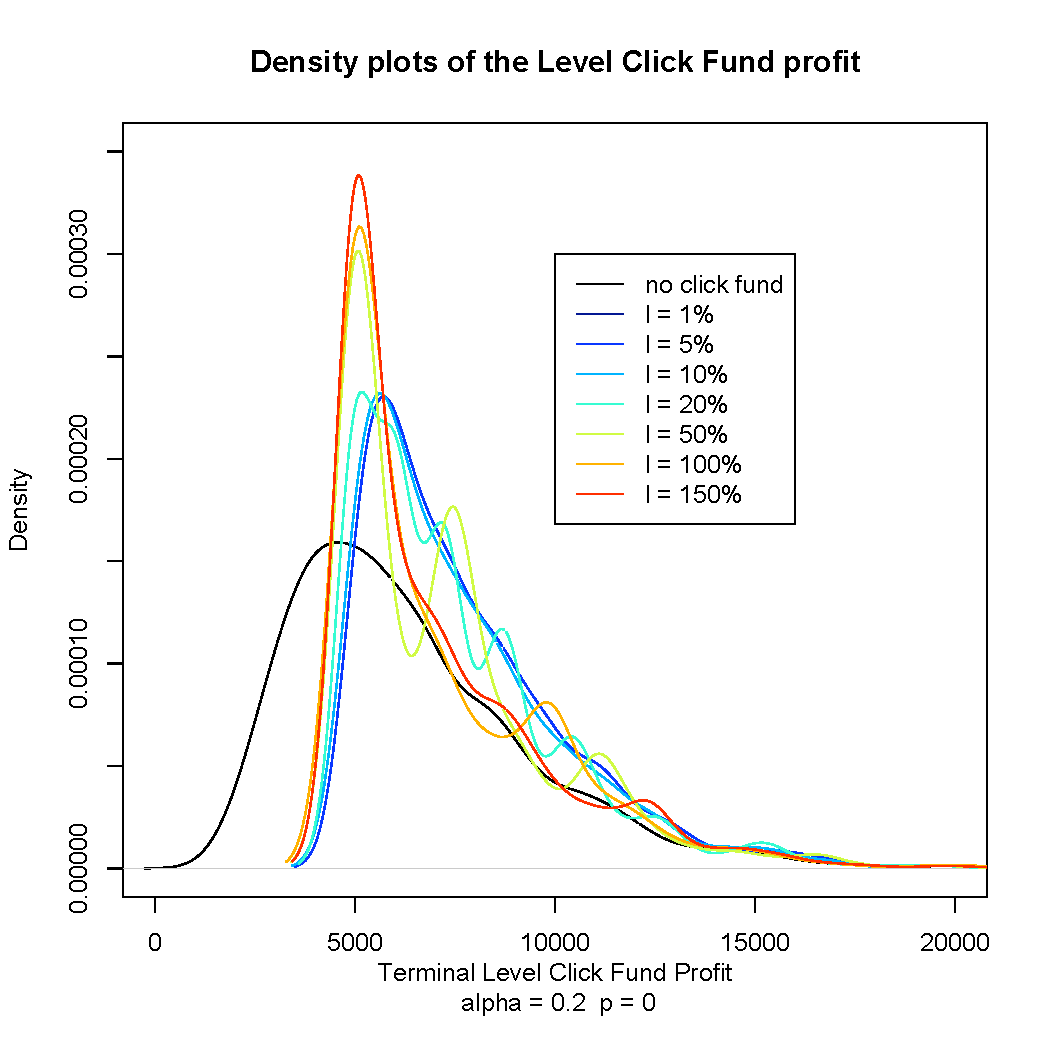
\includegraphics[width=10cm]{dens_lcp_a02p0}
		  \LL}

\ctable[caption={Density plot of the profit of a several level-click funds for
	a stock with a volatility model which has $p = 0.2$ and $\alpha = 0.2$},
		  label={fig:lcfbs2},
		  figure]{c}{}{\FL
		  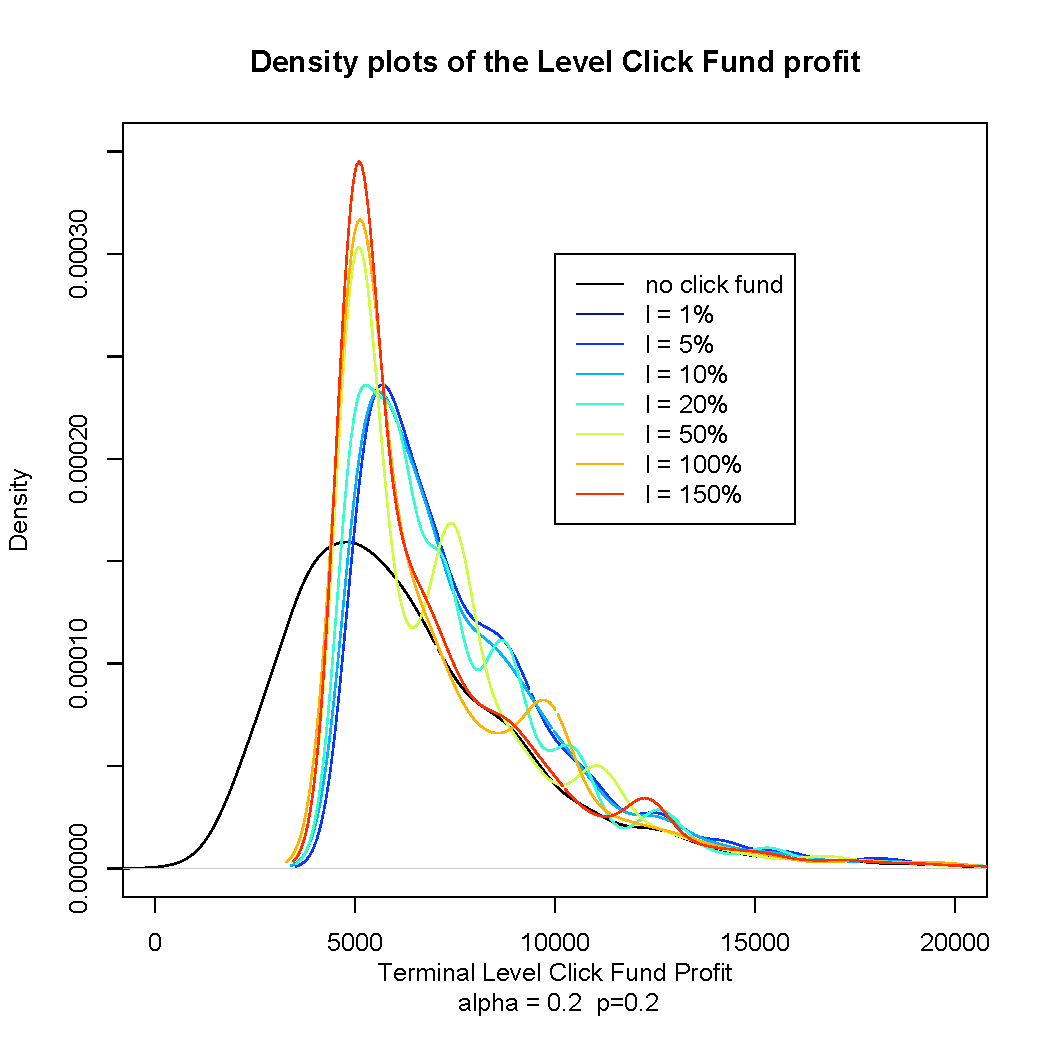
\includegraphics[width=10cm]{dens_lcp_a02p02}
		  \LL}

\ctable[caption={Density plot of the profit of a several level-click funds for
	a stock with a volatility model which has $p = 1$ and $\alpha = 0.2$},
		  label={fig:lcfbs3},
		  figure]{c}{}{\FL
		  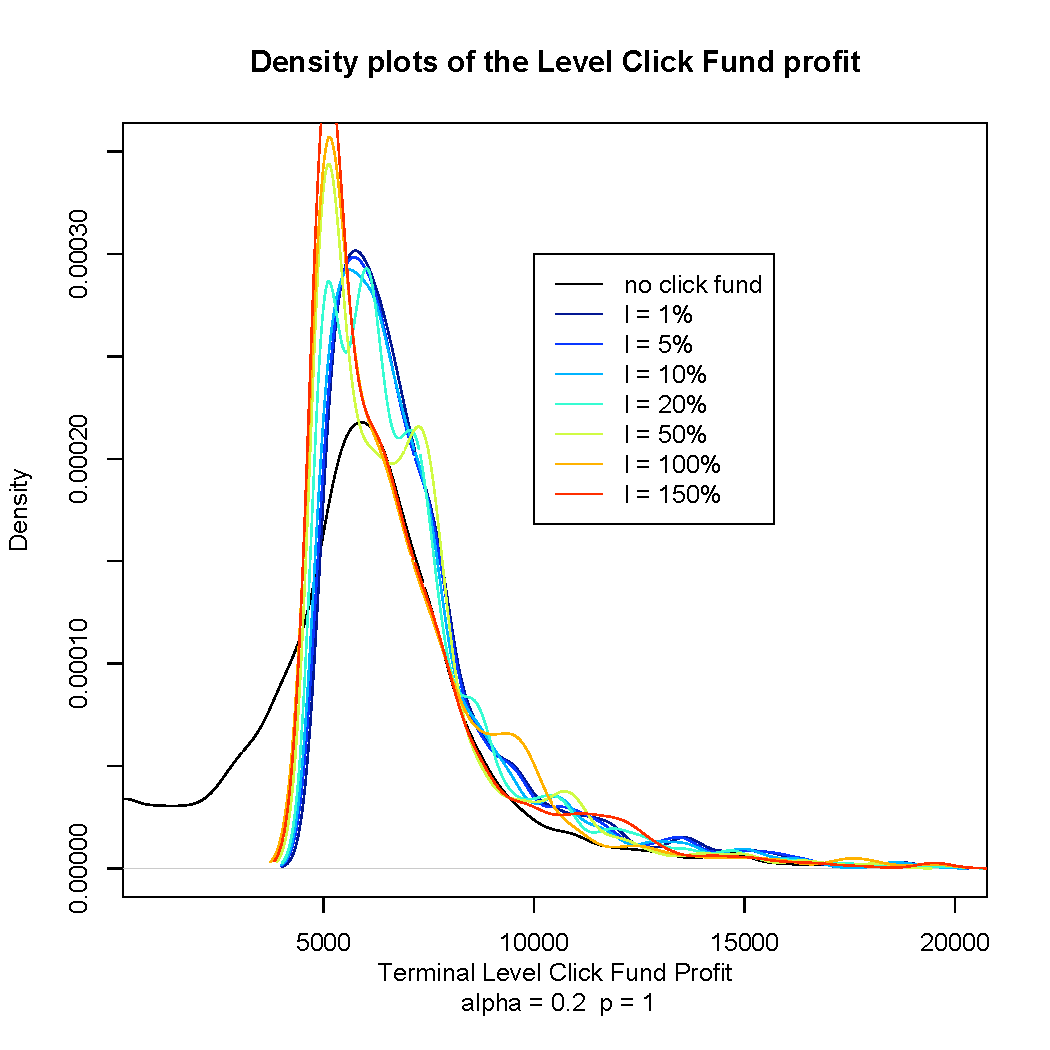
\includegraphics[width=10cm]{dens_lcp_a02p1}
		  \LL}




\bibliographystyle{IEEEtran}
\bibliography{report}
	
\end{document}

% vim: spell spelllang=en:ai
